\subsubsection{\textit{Bubblesort\_aux}}

\paragraph{Lema \ref{lemma:bacount}: \texttt{bubaux\_counts\_n2}:}
\begin{equation*}
    \forall_{l,n,c} bubblesort\_aux\_count(l, c, n)_2 = c + \frac{n^2 + n}{2} \hspace{1cm}, n<|l|, c\in \mathbb{N}
\end{equation*}

\paragraph{Estratégia da prova:} indução forte sobre $|l| + n$. A função
\texttt{bubblesort\_aux\_count} é uma função que faz chamadas
recursivas sobre $l$, e seria correspondente ao próprio Algoritmo
\ref{algo:bubblesort} menos as linhas 5 a 9 (que correspondem melhor com
a função \texttt{bubbling}). A principal questão aqui é que $|l|$
se mantém constante ao longo das chamadas de \texttt{bubblesort\_aux\_count},
portanto uma indução sobre $|l|$ não geraria uma \HI que pudesse ser
instanciada de maneira apropriada.
Uma segunda opção seria realizar a indução sobre $n$, uma vez que ele
é o parâmetro que varia ao longo das chamadas recursivas da função. No
entanto, como $n$ é dependente de $|l|$, foi necessário que a indução
fosse realizada sobre ambos os parâmetros simultaneamente,
daí a escolha de $|l| + n$:
\begin{lstlisting}
  |-------
{1}   FORALL (l: list[nat], n: below[list2finseq(l)`length]) (c: nat):
        bubblesort_aux_count(l, c, n)`2 = c + ((n ^ 2 + n) / 2)

Rule? (measure-induct "length(l) + n" ("l" "n"))
\end{lstlisting} 

A expansão da definição da definição de \texttt{bubbling\_count} após a escolha
da estratégia de prova, resulta em dois casos: o caso base em que
$n=0$ é trivial, pois consiste em provar que $c = c + \frac{n^2 + n}{2}$.
No segundo caso, precisamos provar o sequente:

\begin{lstlisting}
[-1]  (H.I.)
  |-------
{1}   x_2 = 0
{2}   bubblesort_aux_count(bubbling_count(x_1, c, x_2)`1,
                           bubbling_count(x_1, c, x_2)`2, x_2 - 1)`2
       = ((x_2 ^ 2 + x_2) / 2) + c

Rule? (inst -1 "bubbling_count(x_1, c, x_2)`1" "x_2-1")
\end{lstlisting} 

O que permite a instanciação da hipótese de indução da seguinte forma:

\begin{alignat*}{3}
bubblesort\_aux\_count(l, c, n)_2 &= c + ((n ^ 2 + n) / 2) && (h.i.)\\
l &= bubbling\_count(x_1, c, x_2)_1 \\
c &= c \\
n &= x_2-1
\end{alignat*}

A partir deste ponto, a prova novamente se ramifica em duas partes devido
a estratégias ser indução sobre $|l| + n$. No primeiro ramo, que decorre do
do parâmetro $n$, podemos chamar o lema \ref{lemma:bcount} para mostrar que
as chamadas de \texttt{bubbling\_count} incrementam $n$ de forma linear
(Figura \ref{fig:bubaux1}, ramo da esquerda). O segundo ramo decorre
consiste em garantir que estamos instanciando a \HI com valores
estritamente menores do que aqueles no consequente, e prova disso
utiliza o resultado do lema \ref{lemma:blen} que mostra que
$|bubbling\_count(l,c,n)| + n - 1 < |l| + n$, com os valores devidamente
instanciados (Figura \ref{fig:bubaux1}, ramo da direita).

\begin{figure}[H]
    \centering
    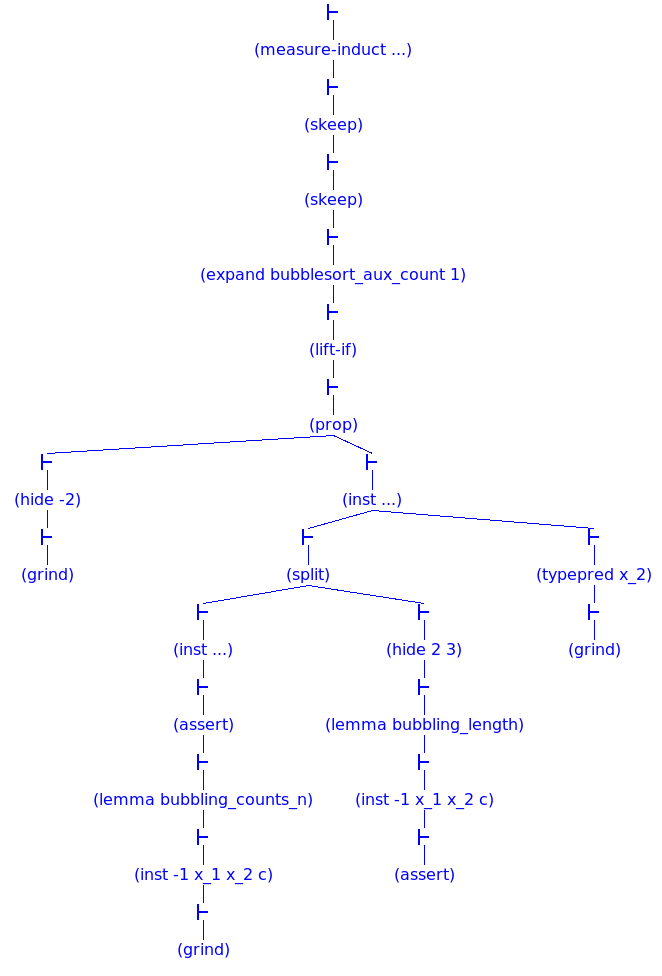
\includegraphics[width=0.75\linewidth,trim={2.5cm 0cm 3.5cm 12cm},clip]{figures/bubaux-counts-n2.png}
    \caption{Para finalizar análise da complexidade de
    \texttt{bubblesort\_aux} usamos os lemas \ref{lemma:bcount}
    e  \ref{lemma:blen} provados anteriormente. O ramo oculto
    ainda mais à direita se refere ao caso base.}
    \label{fig:bubaux1}
\end{figure}

Com isto, temos que a função \texttt{bubblesort\_aux\_count} realiza
$\frac{n^2 + n}{2}$ comparações e portanto é $O(n)$
Da mesma forma que com \texttt{bubbling}, pela restrição de $n<|l|$,
então também é $O(|l|)$. Aqui ainda precisamos mostrar a equivalência
entre os \texttt{bubblesort\_aux} com e sem contador, conforme realizado
a partir do lema a seguir.

\paragraph{Lema \ref{lemma:baequiv}: \texttt{bubblesort\_aux\_equiv}:}
\begin{equation*}
    \forall_{l,n,c} bubblesort\_aux(l, c, n)_1 = bubblesort\_aux\_count(l, c, n)_1    \hspace{1cm}, n<|l|, c\in \mathbb{N}
\end{equation*}

\paragraph{Estratégia da prova:} indução forte sobre $|l| + n$, pela mesma
razão que no lema \ref{lemma:bacount}, já também se refere à função
\texttt{bubblesort\_aux\_count} e \texttt{bubblesort\_aux} apresenta
as mesmas características.

A prova deste lema também requer a expansão da definição de ambas as
funções, \texttt{bubblesort\_aux\_count} e \texttt{bubblesort\_aux}.
Já que essas elas, chamam suas respectivas funções \texttt{bubbling},
podemos instanciar a \HI com a chamada interna de \texttt{bubbling}
de cada uma delas, e completar a prova a partir do lema \ref{lemma:bequiv}.
Da mesma forma que no lema de complexidade \ref{lemma:bacount}, esta
prova também precisa garantir que a instanciação da \HI foi realizada
de maneira adequada, o que também pode ser mostrado usando o resultado
do lema \ref{lemma:blen} sobre o tamanho de $l$ (Figura \ref{fig:bubaux2}).

\begin{figure}[H]
    \centering
    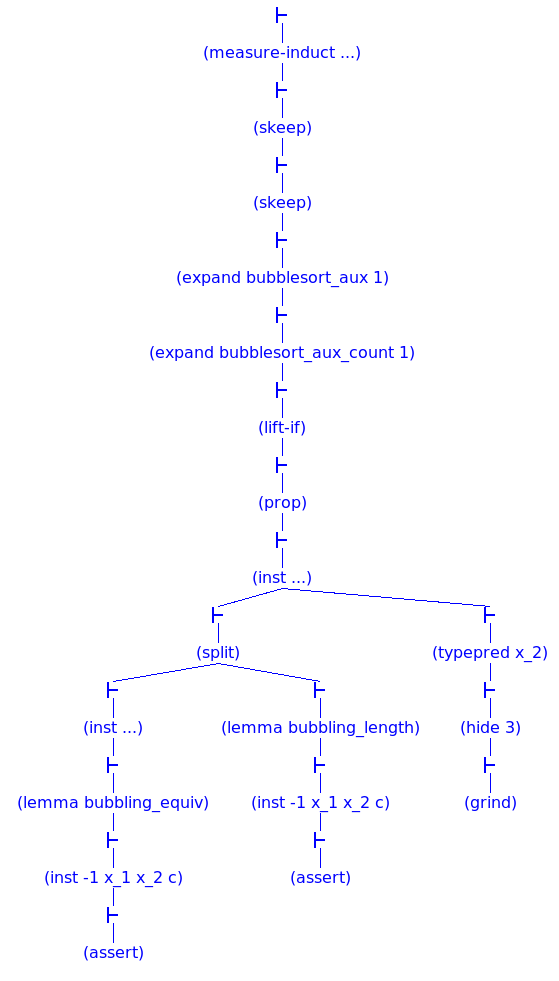
\includegraphics[width=0.75\linewidth,trim={0 0 3.5cm 14cm},clip]{figures/bubblesort-aux-equiv.png}
    \caption{Para finalizar análise de equivalência
    \texttt{bubblesort\_aux} entre \texttt{bubblesort\_aux\_count}
    usamos os lemas \ref{lemma:bequiv} e \ref{lemma:blen}
    provados anteriormente. O ramo oculto mais à direita se
    refere ao caso base.}
    \label{fig:bubaux2}
\end{figure}


